\documentclass[10pt]{article}
\usepackage[T1]{fontenc}
\usepackage[headheight=1.5cm,top=3cm,left=2cm,right=2cm]{geometry}
\usepackage[scaled=0.8]{beramono}
\usepackage{pdflscape}
\usepackage{amsmath}
\usepackage{amsfonts}
\usepackage{helvet}
\usepackage{longtable}
\usepackage{hyperref}
\usepackage{graphicx}

\usepackage{caption}
\usepackage{subcaption}

\usepackage[dvipsnames]{xcolor}
\usepackage{float}
\usepackage{fancyhdr}
\usepackage{multirow}
\usepackage{array}
\newcolumntype{L}[1]{>{\raggedright\let\newline\\\arraybackslash\hspace{0pt}}m{#1}}
\newcolumntype{C}[1]{>{\centering\let\newline\\\arraybackslash\hspace{0pt}}m{#1}}
\newcolumntype{R}[1]{>{\raggedleft\let\newline\\\arraybackslash\hspace{0pt}}m{#1}}

\usepackage{stackengine}
\newcommand\No[1][.13ex]{%
  \setbox0=\hbox{\scalebox{.7}{o}}%
  \setbox2=\hbox{N}%
  N\kern-.05em\stackengine{\dimexpr\ht0-\ht2+#1}{\belowbaseline[-\ht2]{\copy0}}%
    {\rule[-.13ex]{.7\wd0}{.13ex}}%
    {U}{c}{F}{F}{L}%
}

\usepackage{pbox}
%\usepackage{tikz, pgfplots}
\usepackage{pgf,tikz,pgfplots}
\pgfplotsset{compat=1.15}
\usepackage{mathrsfs}
\usetikzlibrary{arrows}
\definecolor{qqqqff}{rgb}{0,0,1}
\definecolor{ffqqqq}{rgb}{1,0,0}
\usepackage{color, colortbl}
\usetikzlibrary{arrows,positioning}
\renewcommand{\familydefault}{\sfdefault}
\setlength{\parindent}{0pt}
\setlength{\parskip}{10pt}
\pagestyle{fancy}
\renewcommand{\headrulewidth}{0.0pt}
\fancyhf{}
\usepackage{lastpage}

\newcommand{\doctitle}{TITLE}
\newcommand{\docauthor}{AUTHOR}

\title{\doctitle}
\author{\docauthor}

\renewcommand{\labelenumii}{\theenumii}
\renewcommand{\theenumii}{\theenumi.\arabic{enumii}.}
\usepackage{enumitem}

\usepackage{listings}

\newcommand{\dev}[1]{{\sc #1}}


\usepackage{longtable}
\usepackage{siunitx}
\usepackage{tabularx}
\newcolumntype{L}[1]{>{\raggedright\arraybackslash}p{#1}} % linksb�ndig mit Breitenangabe
\newcolumntype{C}[1]{>{\centering\arraybackslash}p{#1}} % zentriert mit Breitenangabe
\newcolumntype{R}[1]{>{\raggedleft\arraybackslash}p{#1}} % rechtsb�ndig mit Breitenangabe

% %%% COLOURS FOR LAYERS
% GREEN 81,168,50
% RED Conv 168,50,95
% BLUE Maxpool 50,58,168
% PURPLE upsampling 87,50,168
% RED Concatenate 168,58,50
% Orange Activation 235,128,52
% Turquoise BatchNorm 52,235,174
% PURPLE Additive 174,52,235
\definecolor{InputLayer}{RGB}{52, 220, 235} %light blue

\definecolor{Conv2D}{RGB}{235, 101, 52} % orange/red
\definecolor{Dense}{RGB}{235, 52, 55} %red
\definecolor{BatchNormalization}{RGB}{235, 52, 140} %pink

\definecolor{Activation}{RGB}{92, 52, 235} %blue
\definecolor{Dropout}{RGB}{50, 81, 168} %blue
\definecolor{MaxPooling2D}{RGB}{174, 52, 235} %purple
\definecolor{UpSampling2D}{RGB}{52, 107, 235} %lighter blue

\definecolor{Flatten}{RGB}{50, 168, 70} %Green
\definecolor{Concatenate}{RGB}{81,168,50} %Green
\definecolor{Add}{RGB}{50, 168, 121} % Blueish green
% %%%%%%%%%%%%%%%%%%%%%%
\setcounter{tocdepth}{2}
\begin{document}


$\,$\\[-2ex]
\begin{flushright}
    {\huge{\bf
    \doctitle
    }}\\[1ex]
    {\large
    \docauthor
    }
\end{flushright}

\tableofcontents
% %%%%%%%%%%%%%%%%%%%%%%%%%%%%%%%%%%%%%%%%%%%%%%%%%%%%%%%%%%%%%%%%%%%
\section{Summary}
\begin{tabular}{rrrrrrrr}
    \hline\\[-1.5ex]
    \No{} & Model name & Pretrained & \#Parameters & \#Epochs & Batch size & Test Acc. & Training Acc. \\
    \hline\\[-1.5ex]

    \hyperref[training:1]
             {1} &
    \hyperref[model:MLP2layers]
             {MLP2layers} &
     &
    \num{669706} &
    1
    &
    128 &
    85.82 \% &
    86.78 \%
    \\[4pt]
    \hyperref[training:2]
             {2} &
    \hyperref[model:MLP2layers]
             {MLP2layers} &
     &
    \num{669706} &
    1
    &
    128 &
    86.99 \% &
    86.67 \%
    \\[4pt]
    \hyperref[training:3]
             {3} &
    \hyperref[model:MLP2layers]
             {MLP2layers} &
     &
    \num{669706} &
    1
    &
    128 &
    90.2 \% &
    86.71 \%
    \\[4pt]
    \hline
\end{tabular}
% %%%%%%%%%%%%%%%%%%%%%%%%%%%%%%%%%%%%%%%%%%%%%%%%%%%%%%%%%%%%%%%%%%%
\newpage
% %%%%%%%%%%%%%%%%%%%%%%%%%%%%%%%%%%%%%%%%%%%%%%%%%%%%%%%%%%%%%%%%%%%
\section{Training reports}
    \subsection{Model 1: MLP2layers
                \label{training:1}}
    %
    \paragraph*{Training history} See Figure \ref{fig:results1}.
    \begin{figure}[H]
        \centering
        \begin{subfigure}{.5\textwidth}
            % This file was created by tikzplotlib v0.8.2.
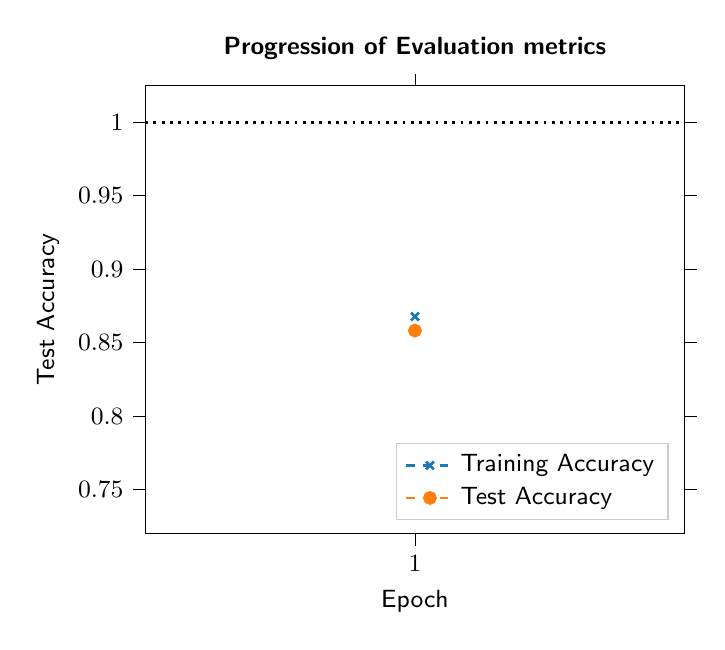
\begin{tikzpicture}

\definecolor{color0}{rgb}{0.12156862745098,0.466666666666667,0.705882352941177}
\definecolor{color1}{rgb}{1,0.498039215686275,0.0549019607843137}

\begin{axis}[
font=\small,
legend cell align={left},
legend style={at={(0.97,0.03)}, anchor=south east, draw=white!80.0!black},
minor xtick={},
minor ytick={},
tick align=outside,
tick pos=both,
title={{\bf Progression of Evaluation metrics}},
x grid style={white!69.01960784313725!black},
xlabel={Epoch},
xmin=0.5, xmax=1.5,
xtick style={color=black},
xtick={1},
y grid style={white!69.01960784313725!black},
ylabel={Test Accuracy},
ymin=0.72, ymax=1.025,
ytick style={color=black},
ytick={0.7,0.75,0.8,0.85,0.9,0.95,1,1.05}
]
\addplot [line width=1.0pt, color0, dashed, mark=x, mark size=2, mark options={solid}]
table {%
1 0.867783333365122
};
\addlegendentry{Training Accuracy}
\addplot [line width=1.0pt, color1, dashed, mark=*, mark size=2, mark options={solid}]
table {%
1 0.8582
};
\addlegendentry{Test Accuracy}
\addplot [line width=1.0pt, black, dotted, forget plot]
table {%
0.5 1
1.5 1
};
\end{axis}

\end{tikzpicture}
            \caption{Accuracy learning process for model \protect\hyperref[training:1]
                        {1}.}
        \end{subfigure}%
        \hfill%
        \begin{subfigure}{.5\textwidth}
            % This file was created by tikzplotlib v0.8.2.
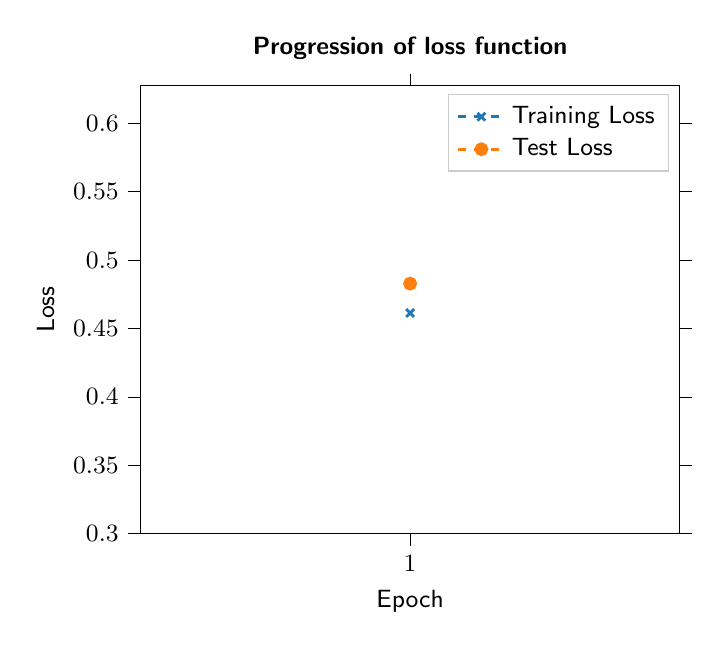
\begin{tikzpicture}

\definecolor{color0}{rgb}{0.12156862745098,0.466666666666667,0.705882352941177}
\definecolor{color1}{rgb}{1,0.498039215686275,0.0549019607843137}

\begin{axis}[
font=\small,
legend cell align={left},
legend style={draw=white!80.0!black},
minor xtick={},
minor ytick={},
tick align=outside,
tick pos=both,
title={{\bf Progression of loss function}},
x grid style={white!69.01960784313725!black},
xlabel={Epoch},
xmin=0.5, xmax=1.5,
xtick style={color=black},
xtick={1},
y grid style={white!69.01960784313725!black},
ylabel={Loss},
ymin=0.3, ymax=0.627594272327423,
ytick style={color=black},
ytick={0.3,0.35,0.4,0.45,0.5,0.55,0.6,0.65}
]
\addplot [line width=1.0pt, color0, dashed, mark=x, mark size=2, mark options={solid}]
table {%
1 0.461344637664159
};
\addlegendentry{Training Loss}
\addplot [line width=1.0pt, color1, dashed, mark=*, mark size=2, mark options={solid}]
table {%
1 0.482764824867249
};
\addlegendentry{Test Loss}
\end{axis}

\end{tikzpicture}
            \caption{Loss learning process for model \protect\hyperref[training:1]
                        {1}.}
        \end{subfigure}
        \par\bigskip
        \begin{subfigure}{.5\textwidth}
            % This file was created by tikzplotlib v0.8.2.
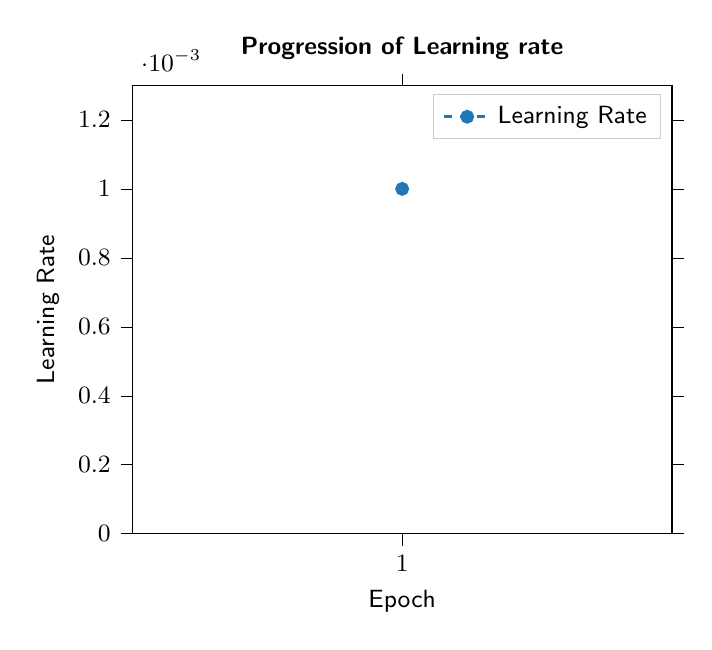
\begin{tikzpicture}

\definecolor{color0}{rgb}{0.12156862745098,0.466666666666667,0.705882352941177}

\begin{axis}[
font=\small,
legend cell align={left},
legend style={draw=white!80.0!black},
minor xtick={},
minor ytick={},
tick align=outside,
tick pos=both,
title={{\bf Progression of Learning rate}},
x grid style={white!69.01960784313725!black},
xlabel={Epoch},
xmin=0.5, xmax=1.5,
xtick style={color=black},
xtick={1},
y grid style={white!69.01960784313725!black},
ylabel={Learning Rate},
ymin=0, ymax=0.0013,
ytick style={color=black},
ytick={0,0.0002,0.0004,0.0006,0.0008,0.001,0.0012,0.0014}
]
\addplot [line width=1.0pt, color0, dashed, mark=*, mark size=2, mark options={solid}]
table {%
1 0.001
};
\addlegendentry{Learning Rate}
\end{axis}

\end{tikzpicture}
            \caption{Learning rate per epoch for model \protect\hyperref[training:1]
                        {1}.}
        \end{subfigure}%
        \caption{Training and evaluation metrics for model  \protect\hyperref[training:1]
                    {1}.
                \label{fig:results1}}
    \end{figure}

    \subsubsection*{Dataset}
    \begin{description}
        \item[Name] MNIST
        \item[Train-Test-Dev split:] {\it Training set:}
        60000,
        {\it Test set:}
        10000,
        {\it Dev set:}
        0,
        \item[Image size] [28, 28]


    \end{description}
    %
    \subsubsection*{Training}
    \begin{description}
        \item[Number of epochs] 1
        \item[Optimizer] Rmsprop \\
            0.01\\
        \item[Learning rate] 0.001
        \item[Loss] Categorical crossentropy
        \item[Batch size] 128
        \item[Shuffle] Yes
        \item[Training time] 4 sec
    \end{description}
    %
    \subsubsection*{Platform}
    \begin{description}
        \item[Weights exported to path] weights\textbackslash MLP2layers\_1ep\_MNIST.h5
        \item[Device used] GPU (GeForce GTX 1060 6GB)
        \item[CPU] Intel(R) Xeon(R) CPU E3-1245 v5 @ 3.50GHz,
                   X86\_64
        \item[Python Version] 3.7.2.final.0 (64 bit)
        \item[Keras Version] 2.2.5 (Backend: tensorflow)
        \item[Tensorflow Version] 1.14.0
        \item[Timestamp] 25.09.2019 at 13:50
    \end{description}
    \subsection{Model 2: MLP2layers
                \label{training:2}}
    %
    \paragraph*{Training history} See Figure \ref{fig:results2}.
    \begin{figure}[H]
        \centering
        \begin{subfigure}{.5\textwidth}
            % This file was created by tikzplotlib v0.8.2.
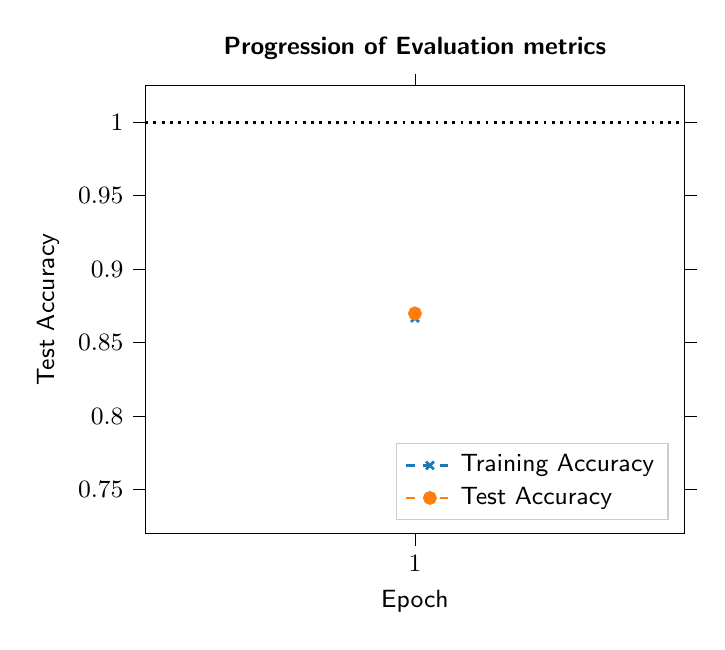
\begin{tikzpicture}

\definecolor{color0}{rgb}{0.12156862745098,0.466666666666667,0.705882352941177}
\definecolor{color1}{rgb}{1,0.498039215686275,0.0549019607843137}

\begin{axis}[
font=\small,
legend cell align={left},
legend style={at={(0.97,0.03)}, anchor=south east, draw=white!80.0!black},
minor xtick={},
minor ytick={},
tick align=outside,
tick pos=both,
title={{\bf Progression of Evaluation metrics}},
x grid style={white!69.01960784313725!black},
xlabel={Epoch},
xmin=0.5, xmax=1.5,
xtick style={color=black},
xtick={1},
y grid style={white!69.01960784313725!black},
ylabel={Test Accuracy},
ymin=0.72, ymax=1.025,
ytick style={color=black},
ytick={0.7,0.75,0.8,0.85,0.9,0.95,1,1.05}
]
\addplot [line width=1.0pt, color0, dashed, mark=x, mark size=2, mark options={solid}]
table {%
1 0.866733333365122
};
\addlegendentry{Training Accuracy}
\addplot [line width=1.0pt, color1, dashed, mark=*, mark size=2, mark options={solid}]
table {%
1 0.8699
};
\addlegendentry{Test Accuracy}
\addplot [line width=1.0pt, black, dotted, forget plot]
table {%
0.5 1
1.5 1
};
\end{axis}

\end{tikzpicture}
            \caption{Accuracy learning process for model \protect\hyperref[training:2]
                        {2}.}
        \end{subfigure}%
        \hfill%
        \begin{subfigure}{.5\textwidth}
            % This file was created by tikzplotlib v0.8.2.
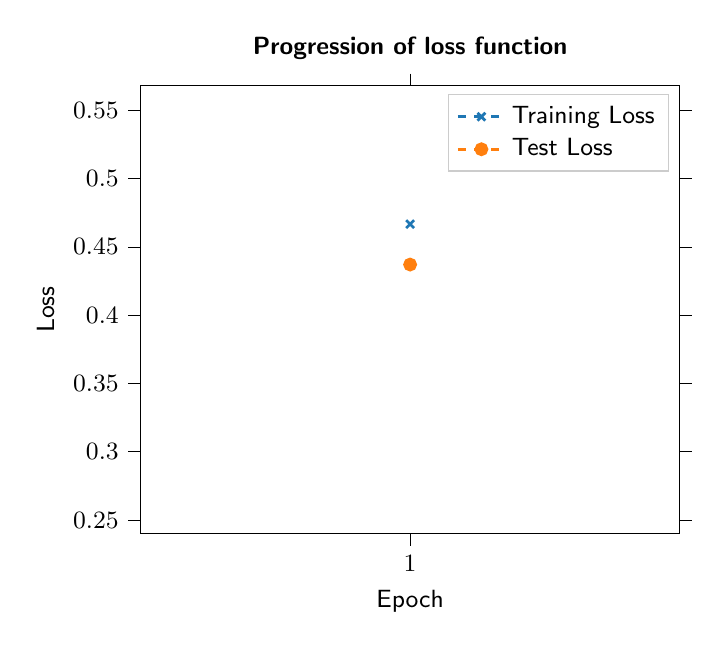
\begin{tikzpicture}

\definecolor{color0}{rgb}{0.12156862745098,0.466666666666667,0.705882352941177}
\definecolor{color1}{rgb}{1,0.498039215686275,0.0549019607843137}

\begin{axis}[
font=\small,
legend cell align={left},
legend style={draw=white!80.0!black},
minor xtick={},
minor ytick={},
tick align=outside,
tick pos=both,
title={{\bf Progression of loss function}},
x grid style={white!69.01960784313725!black},
xlabel={Epoch},
xmin=0.5, xmax=1.5,
xtick style={color=black},
xtick={1},
y grid style={white!69.01960784313725!black},
ylabel={Loss},
ymin=0.24, ymax=0.568110058338642,
ytick style={color=black},
ytick={0.2,0.25,0.3,0.35,0.4,0.45,0.5,0.55,0.6}
]
\addplot [line width=1.0pt, color0, dashed, mark=x, mark size=2, mark options={solid}]
table {%
1 0.466604991785685
};
\addlegendentry{Training Loss}
\addplot [line width=1.0pt, color1, dashed, mark=*, mark size=2, mark options={solid}]
table {%
1 0.437007737183571
};
\addlegendentry{Test Loss}
\end{axis}

\end{tikzpicture}
            \caption{Loss learning process for model \protect\hyperref[training:2]
                        {2}.}
        \end{subfigure}
        \par\bigskip
        \begin{subfigure}{.5\textwidth}
            % This file was created by tikzplotlib v0.8.2.
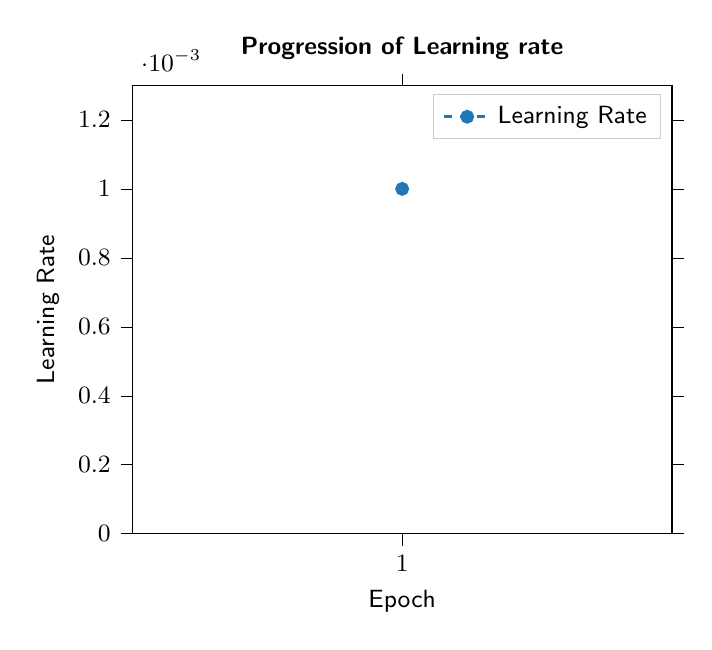
\begin{tikzpicture}

\definecolor{color0}{rgb}{0.12156862745098,0.466666666666667,0.705882352941177}

\begin{axis}[
font=\small,
legend cell align={left},
legend style={draw=white!80.0!black},
minor xtick={},
minor ytick={},
tick align=outside,
tick pos=both,
title={{\bf Progression of Learning rate}},
x grid style={white!69.01960784313725!black},
xlabel={Epoch},
xmin=0.5, xmax=1.5,
xtick style={color=black},
xtick={1},
y grid style={white!69.01960784313725!black},
ylabel={Learning Rate},
ymin=0, ymax=0.0013,
ytick style={color=black},
ytick={0,0.0002,0.0004,0.0006,0.0008,0.001,0.0012,0.0014}
]
\addplot [line width=1.0pt, color0, dashed, mark=*, mark size=2, mark options={solid}]
table {%
1 0.001
};
\addlegendentry{Learning Rate}
\end{axis}

\end{tikzpicture}
            \caption{Learning rate per epoch for model \protect\hyperref[training:2]
                        {2}.}
        \end{subfigure}%
        \caption{Training and evaluation metrics for model  \protect\hyperref[training:2]
                    {2}.
                \label{fig:results2}}
    \end{figure}

    \subsubsection*{Dataset}
    \begin{description}
        \item[Name] MNIST
        \item[Train-Test-Dev split:] {\it Training set:}
        60000,
        {\it Test set:}
        10000,
        {\it Dev set:}
        0,
        \item[Image size] [28, 28]


    \end{description}
    %
    \subsubsection*{Training}
    \begin{description}
        \item[Number of epochs] 1
        \item[Optimizer] Rmsprop \\
            0.01\\
        \item[Learning rate] 0.001
        \item[Loss] Categorical crossentropy
        \item[Batch size] 128
        \item[Shuffle] Yes
        \item[Training time] 4 sec
    \end{description}
    %
    \subsubsection*{Platform}
    \begin{description}
        \item[Weights exported to path] weights\textbackslash MLP2layers\_1ep\_MNIST.h5
        \item[Device used] GPU (GeForce GTX 1060 6GB)
        \item[CPU] Intel(R) Xeon(R) CPU E3-1245 v5 @ 3.50GHz,
                   X86\_64
        \item[Python Version] 3.7.2.final.0 (64 bit)
        \item[Keras Version] 2.2.5 (Backend: tensorflow)
        \item[Tensorflow Version] 1.14.0
        \item[Timestamp] 25.09.2019 at 13:52
    \end{description}
    \subsection{Model 3: MLP2layers
                \label{training:3}}
    %
    \paragraph*{Training history} See Figure \ref{fig:results3}.
    \begin{figure}[H]
        \centering
        \begin{subfigure}{.5\textwidth}
            % This file was created by tikzplotlib v0.8.2.
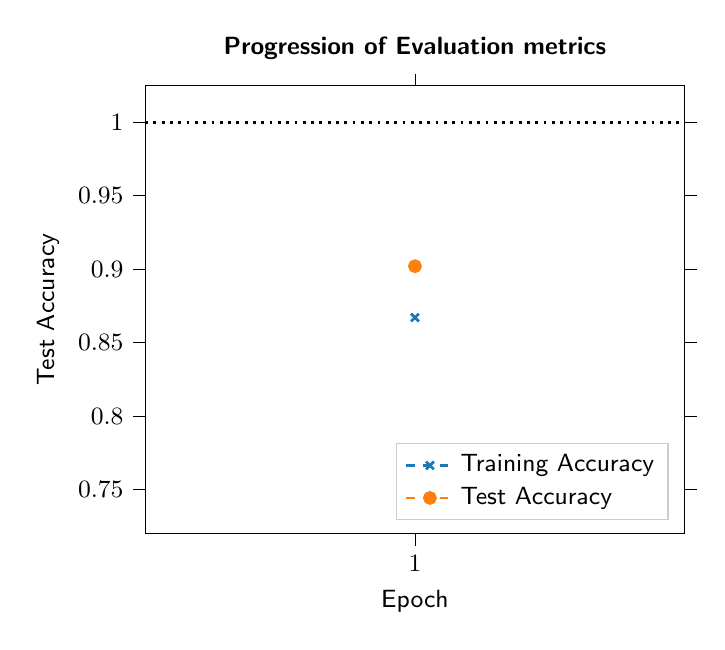
\begin{tikzpicture}

\definecolor{color0}{rgb}{0.12156862745098,0.466666666666667,0.705882352941177}
\definecolor{color1}{rgb}{1,0.498039215686275,0.0549019607843137}

\begin{axis}[
font=\small,
legend cell align={left},
legend style={at={(0.97,0.03)}, anchor=south east, draw=white!80.0!black},
minor xtick={},
minor ytick={},
tick align=outside,
tick pos=both,
title={{\bf Progression of Evaluation metrics}},
x grid style={white!69.01960784313725!black},
xlabel={Epoch},
xmin=0.5, xmax=1.5,
xtick style={color=black},
xtick={1},
y grid style={white!69.01960784313725!black},
ylabel={Test Accuracy},
ymin=0.72, ymax=1.025,
ytick style={color=black},
ytick={0.7,0.75,0.8,0.85,0.9,0.95,1,1.05}
]
\addplot [line width=1.0pt, color0, dashed, mark=x, mark size=2, mark options={solid}]
table {%
1 0.867083333333333
};
\addlegendentry{Training Accuracy}
\addplot [line width=1.0pt, color1, dashed, mark=*, mark size=2, mark options={solid}]
table {%
1 0.902
};
\addlegendentry{Test Accuracy}
\addplot [line width=1.0pt, black, dotted, forget plot]
table {%
0.5 1
1.5 1
};
\end{axis}

\end{tikzpicture}
            \caption{Accuracy learning process for model \protect\hyperref[training:3]
                        {3}.}
        \end{subfigure}%
        \hfill%
        \begin{subfigure}{.5\textwidth}
            % This file was created by tikzplotlib v0.8.2.
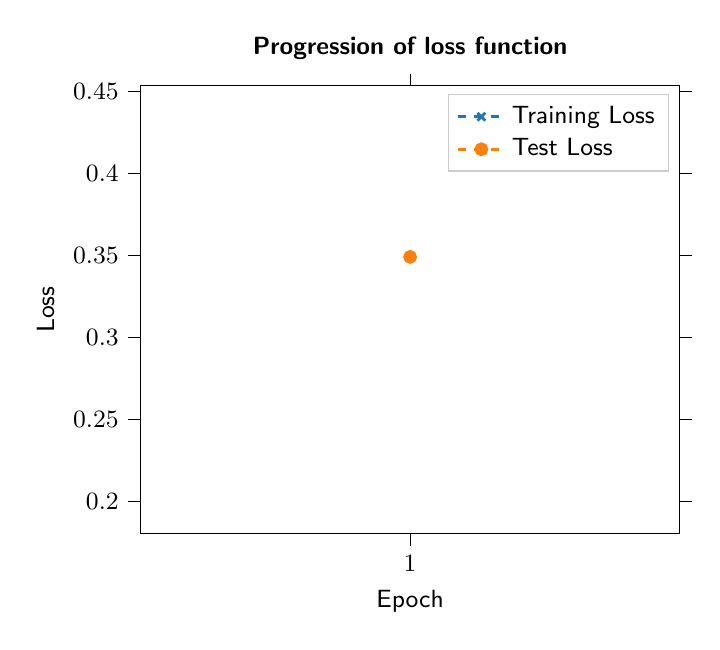
\begin{tikzpicture}

\definecolor{color0}{rgb}{0.12156862745098,0.466666666666667,0.705882352941177}
\definecolor{color1}{rgb}{1,0.498039215686275,0.0549019607843137}

\begin{axis}[
font=\small,
legend cell align={left},
legend style={draw=white!80.0!black},
minor xtick={},
minor ytick={},
tick align=outside,
tick pos=both,
title={{\bf Progression of loss function}},
x grid style={white!69.01960784313725!black},
xlabel={Epoch},
xmin=0.5, xmax=1.5,
xtick style={color=black},
xtick={1},
y grid style={white!69.01960784313725!black},
ylabel={Loss},
ymin=0.18, ymax=0.453740831608772,
ytick style={color=black},
ytick={0.15,0.2,0.25,0.3,0.35,0.4,0.45,0.5}
]
\addplot [line width=1.0pt, color0, dashed, mark=x, mark size=2, mark options={solid}]
table {%
1 0.465589972003301
};
\addlegendentry{Training Loss}
\addplot [line width=1.0pt, color1, dashed, mark=*, mark size=2, mark options={solid}]
table {%
1 0.349031408929825
};
\addlegendentry{Test Loss}
\end{axis}

\end{tikzpicture}
            \caption{Loss learning process for model \protect\hyperref[training:3]
                        {3}.}
        \end{subfigure}
        \par\bigskip
        \begin{subfigure}{.5\textwidth}
            % This file was created by tikzplotlib v0.8.2.
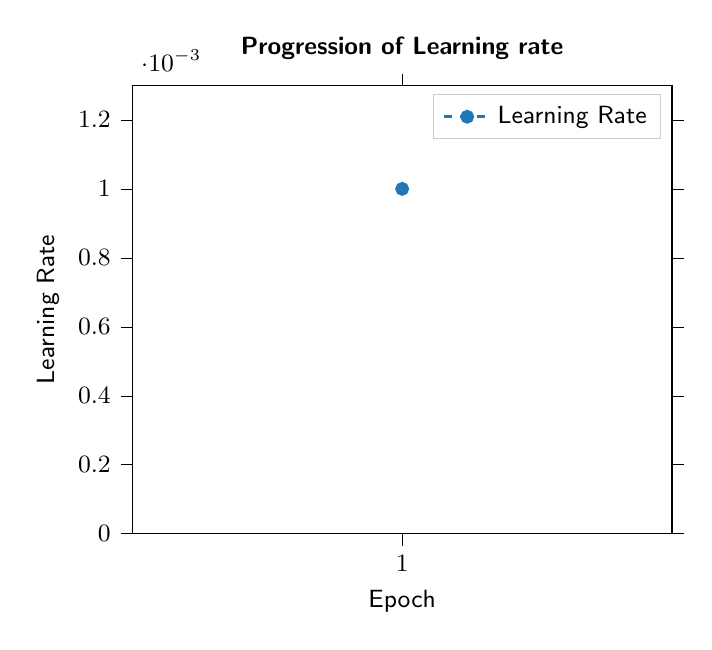
\begin{tikzpicture}

\definecolor{color0}{rgb}{0.12156862745098,0.466666666666667,0.705882352941177}

\begin{axis}[
font=\small,
legend cell align={left},
legend style={draw=white!80.0!black},
minor xtick={},
minor ytick={},
tick align=outside,
tick pos=both,
title={{\bf Progression of Learning rate}},
x grid style={white!69.01960784313725!black},
xlabel={Epoch},
xmin=0.5, xmax=1.5,
xtick style={color=black},
xtick={1},
y grid style={white!69.01960784313725!black},
ylabel={Learning Rate},
ymin=0, ymax=0.0013,
ytick style={color=black},
ytick={0,0.0002,0.0004,0.0006,0.0008,0.001,0.0012,0.0014}
]
\addplot [line width=1.0pt, color0, dashed, mark=*, mark size=2, mark options={solid}]
table {%
1 0.001
};
\addlegendentry{Learning Rate}
\end{axis}

\end{tikzpicture}
            \caption{Learning rate per epoch for model \protect\hyperref[training:3]
                        {3}.}
        \end{subfigure}%
        \caption{Training and evaluation metrics for model  \protect\hyperref[training:3]
                    {3}.
                \label{fig:results3}}
    \end{figure}

    \subsubsection*{Dataset}
    \begin{description}
        \item[Name] MNIST
        \item[Train-Test-Dev split:] {\it Training set:}
        60000,
        {\it Test set:}
        10000,
        {\it Dev set:}
        0,
        \item[Image size] [28, 28]


    \end{description}
    %
    \subsubsection*{Training}
    \begin{description}
        \item[Number of epochs] 1
        \item[Optimizer] Rmsprop \\
            0.01\\
        \item[Learning rate] 0.001
        \item[Loss] Categorical crossentropy
        \item[Batch size] 128
        \item[Shuffle] Yes
        \item[Training time] 5 sec
    \end{description}
    %
    \subsubsection*{Platform}
    \begin{description}
        \item[Weights exported to path] weights\textbackslash MLP2layers\_1ep\_MNIST.h5
        \item[Device used] GPU (GeForce GTX 1060 6GB)
        \item[CPU] Intel(R) Xeon(R) CPU E3-1245 v5 @ 3.50GHz,
                   X86\_64
        \item[Python Version] 3.7.2.final.0 (64 bit)
        \item[Keras Version] 2.2.5 (Backend: tensorflow)
        \item[Tensorflow Version] 1.14.0
        \item[Timestamp] 25.09.2019 at 13:53
    \end{description}
% %%%%%%%%%%%%%%%%%%%%%%%%%%%%%%%%%%%%%%%%%%%%%%%%%%%%%%%%%%%%%%%%%%%
\newpage
% %%%%%%%%%%%%%%%%%%%%%%%%%%%%%%%%%%%%%%%%%%%%%%%%%%%%%%%%%%%%%%%%%%%
\section{Model Architectures}
\subsection{MLP2layers
            \label{model:MLP2layers}
            }
\paragraph{Used in \No{}:}
    \hyperref[training:1]
             {1},
    \hyperref[training:2]
             {2},
    \hyperref[training:3]
             {3}
\vspace{-2ex}
%
\paragraph{Model summary:}$\,$\\
\begin{longtable}{rR{.22\textwidth}cL{.22\textwidth}rL{.22\textwidth}}
    \hline\\[-1.5ex]
    \No{} &
    Layer (Type) &
    Output shape &
    Config &
    \#Parameters &
    Inbound layers\\
    \hline\\
    \endhead
        0
        &
        \color{InputLayer}{
        input\_1}
        \color{InputLayer}{
        (InputLayer)}
        &
        (28, 28, 1)
        &
        &
        \num{0}
        &
        \\
        \hline\\[-1.5ex]
        1
        &
        \color{Flatten}{
        flatten\_1}
        \color{Flatten}{
        (Flatten)}
        &
        (784,)
        &
            Parameters of layers of type Flatten not implemented.
        &
        \num{0}
        &
        \color{InputLayer}{
            input\_1}
        \\
        \hline\\[-1.5ex]
        2
        &
        \color{Dense}{
        dense\_1}
        \color{Dense}{
        (Dense)}
        &
        (512,)
        &
            Parameters of layers of type Dense not implemented.
        &
        \num{401920}
        &
        \color{Flatten}{
            flatten\_1}
        \\
        \hline\\[-1.5ex]
        3
        &
        \color{Dropout}{
        dropout\_1}
        \color{Dropout}{
        (Dropout)}
        &
        (512,)
        &
            Parameters of layers of type Dropout not implemented.
        &
        \num{0}
        &
        \color{Dense}{
            dense\_1}
        \\
        \hline\\[-1.5ex]
        4
        &
        \color{Dense}{
        dense\_2}
        \color{Dense}{
        (Dense)}
        &
        (512,)
        &
            Parameters of layers of type Dense not implemented.
        &
        \num{262656}
        &
        \color{Dropout}{
            dropout\_1}
        \\
        \hline\\[-1.5ex]
        5
        &
        \color{Dropout}{
        dropout\_2}
        \color{Dropout}{
        (Dropout)}
        &
        (512,)
        &
            Parameters of layers of type Dropout not implemented.
        &
        \num{0}
        &
        \color{Dense}{
            dense\_2}
        \\
        \hline\\[-1.5ex]
        6
        &
        \color{Dense}{
        dense\_3}
        \color{Dense}{
        (Dense)}
        &
        (10,)
        &
            Parameters of layers of type Dense not implemented.
        &
        \num{5130}
        &
        \color{Dropout}{
            dropout\_2}
        \\
        \hline\\[-1.5ex]
\end{longtable}
\newpage
% %%%%%%%%%%%%%%%%%%%%%%%%%%%%%%%%%%%%%%%%%%%%%%%%%%%%%%%%%%%%%%%%%%%

\end{document}